\subsubsection{Argo} 

\paragraph{Overview} 

The Argo project~\cite{perarnau2017argo} is building portable, open source system software that improves
the performance and scalability and provides increased functionality to
Exascale applications and runtime systems.

We focus on four areas of the OS/R stack where the need from the ECP
applications and facilities is perceived to be the most urgent:
1) support for hierarchical memory;
2) dynamic and hierarchical power management to meet performance
targets;
3) containers for managing resources within a node; and
4) internode interfaces for collectively managing resources across groups
of nodes.


\paragraph{Key Challenges}

Many ECP applications have a complex runtime structure, ranging from in
situ data analysis, through an ensemble of largely independent individual
subjobs, to arbitrarily complex workflow structures~\cite{dreher2017situ}.  At the same time, HPC
hardware complexity increases as well, from deeper memory hierarchies
encompassing on-package DRAM and byte-addressable NVRAM, to heterogeneous
compute resources and performance changing dynamically based on
power/thermal constraints.

To meet the emerging needs of ECP workloads while providing optimal
performance and resilience, the compute, memory, and interconnect resources
must be managed in cooperation with applications and runtime systems; yet
existing resource management solutions lack the necessary capabilities and
vendors are reluctant to innovate in this space in the absence of clear
directions from the community.


\paragraph{Solution Strategy}

Our approach is to augment and optimize for HPC the existing open source
offerings provided by vendors. We are working with ECP applications and
runtime systems to distill the needed new interfaces and to build, test,
and evaluate the newly implemented functionality with ECP workloads.  This
needs to be done in cooperation with facilities, who can provide early
hardware testbeds where the newly implemented functionality can be
demonstrated to show benefits, tested at scale, and matured.  Over the
years we have cultivated an excellent relationship with the vendors
providing HPC platforms because our approach has been to augment and
improve, rather than develop our own OS/R from scratch.  IBM, Cray, and
Intel are eager to integrate the components we develop for ECP that can
help applications.

Our work in each area focuses on the following:

\begin{enumerate}

\item \textbf{Hierarchical memory:} Incorporate NVRAM into the memory hierarchy
using UMap: a user-space \texttt{mmap} replacement for out-of-core data,
leveraging recent \texttt{userfaultfd} mechanism of the Linux kernel for page fault
handling, featuring application-class specific prefetching and eviction
algorithms.  Expose deep DRAM hierarchy by treating high-bandwidth memory
(MCDRAM, HBM) as a scratchpad~\cite{perarnau2016exploring}, managed by the Argonne Memory Library (AML),
which provides applications with asynchronous memory migration
between memory tiers and other convenience mechanisms.

\item \textbf{Power management:}
\emph{PowerStack} will explore hierarchical interfaces for power management
at three specific
levels~\cite{Ellsworth:argo,ellsworth_e2sc2016,patki2016,sakamoto2017}: the
global level of batch job schedulers (which we refer to as the Global
Resource Manager or GRM), the enclave level of job-level runtime systems
(open-source solution of Intel GEOPM and the ECP Power Steering project
will be leveraged here), and the node-level through measurement and control
mechanisms integrated with the NRM (described below).
At the node level, we will develop low-level, vendor-specific 
monitoring/controlling capabilities to monitor power/energy consumption,
core temperature and other hardware status~\cite{osti_1353371,zhang2015minimizing}, and control the hardware power
capping and the CPU frequencies. 

\item \textbf{Containers:} Develop a Node Resource Manager (NRM) that leverages
technologies underlying modern container runtimes
(primarily \texttt{cgroups}) to partition resources on compute nodes~\cite{zounmevo2015container},
arbitrating between application components and runtime services.

\item \textbf{Hierarchical resource management:} Develop a set of distributed
services and user-facing interfaces~\cite{perarnau2015distributed} to allow applications and runtimes to
resize, subdivide, and reconfigure their resources inside a job.  Provide
the enclave abstraction: recursive groups of nodes that are managed as a
single entity; those enclaves can then be used to launch new services or to
create subjobs that can communicate with each other.
\end{enumerate}


\paragraph{Recent Progress}

We identified initial representative ECP applications and benchmarks of
interest, focusing in particular on characteristics such as: coupled codes
consisting of multiple components, memory-intensive codes that do not fit
well in DRAM or that are bandwidth-bound, and codes with dynamically
changing resource requirements.
%We interfaced (either face-to-face or via
%teleconferencing) with the representatives of the following projects:
%NWChemEx, PaRSEC, CANDLE, GAMESS, MPI teams, PETSc, SOLLVE, SICM, PowerRT,
%and Flux.

We designed and developed an API between Node Power and Node
Resource Manager (NRM), which in turn allows Global Resource
Manager (GRM) to control and monitor power and other node-local
resources. Additionally, we studied the effect of power capping on
different applications using the NodePower API and developed power
regression models required for a demand-response policy, which may be
added to the GRM in future.

We developed Yggdrasil, a resource event reactor that provides the enclave
abstraction.  It can use standard HPC schedulers such as SLURM or Flux as a
backend.

We developed the initial, centralized version of the Global Resource
Manager (GRM) providing a hierarchical framework for power control.  We
enhanced existing PowSched codebase to use the power controller in the node
OS to acquire node local power data and adjust the power caps. We also developed a variation-aware
scheduler to address manufacturing variability under power constraints with Flux infrastructure, 
and extended SLURM to support power scheduling plugins to enable our upcoming GRM 
milestones. 

We designed and developed the first version of the unified Node
Resource Manager.  The NRM provides high level of control over node
resources, including initial allocation at job launch and dynamic
reallocation at the request of the application and other services.
The initial set of
managed resources includes CPU cores and memory; they can be allocated to
application components via a container abstraction, which is used to describe
partitions of physical resources (to decrease interference),
and more.

We developed the first stable version of UMap, the user-space memory map
page fault handler for NVRAM. 
UMap handler maps application
threads' virtual address ranges to persistent data sets, transparently
pages in active pages and evicts unused pages.  We evaluated the costs and
overheads of various approaches and characterized end-to-end performance
for simple I/O intensive applications.

We designed AML, a memory library for explicit management of deep memory
architectures, and validated it on Intel's Knights Landing. Its main
feature is a scratchpad API, allowing applications to implement algorithms
similar to out-of-core for deep memory.
We provided multiple optimized versions of memory migration facilities,
ranging from a regular copy to a transparent move of memory pages, using
synchronous and asynchronous interfaces and single- and multithreaded
backends.

\begin{figure}[h]
\centering
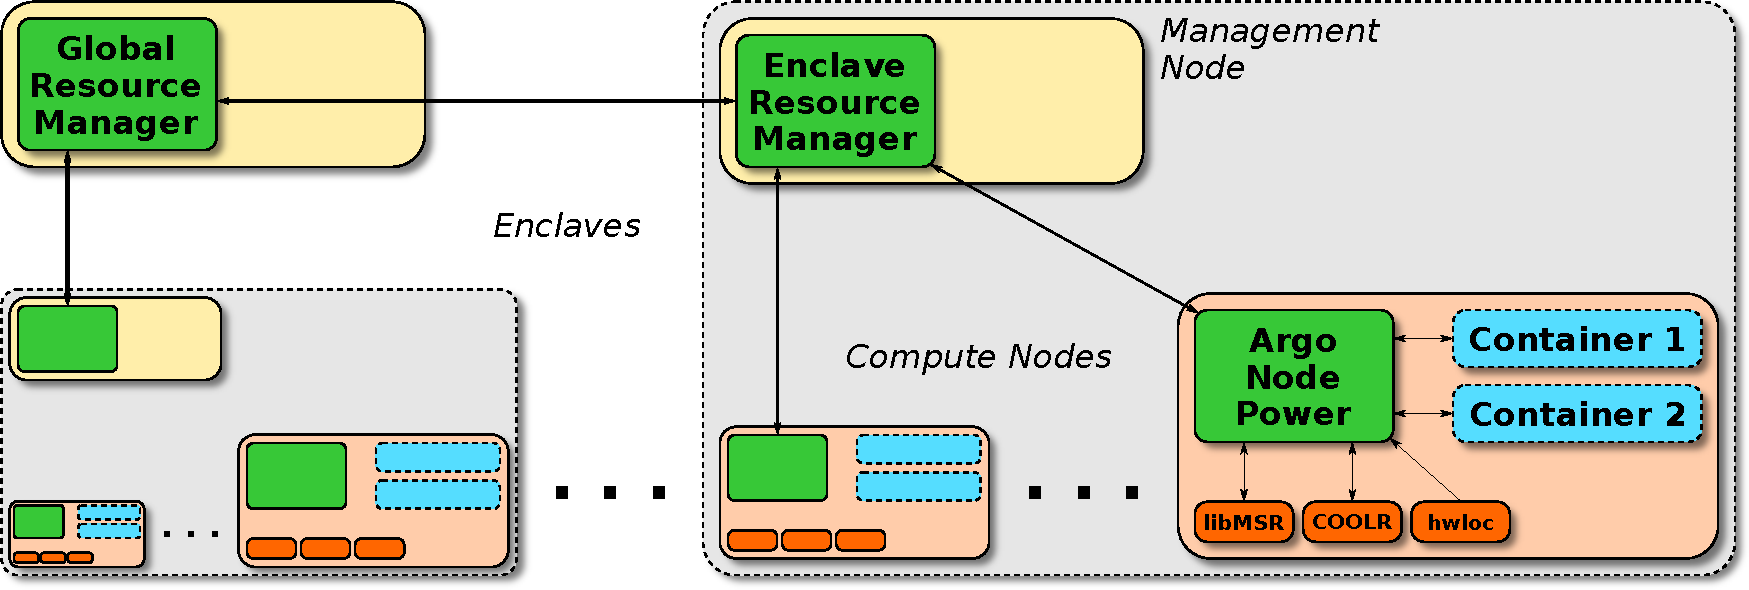
\includegraphics[height=.15\textheight]{projects/2.3.5-Ecosystem/2.3.5.05-Argo/argo-global}\hspace{1em}%
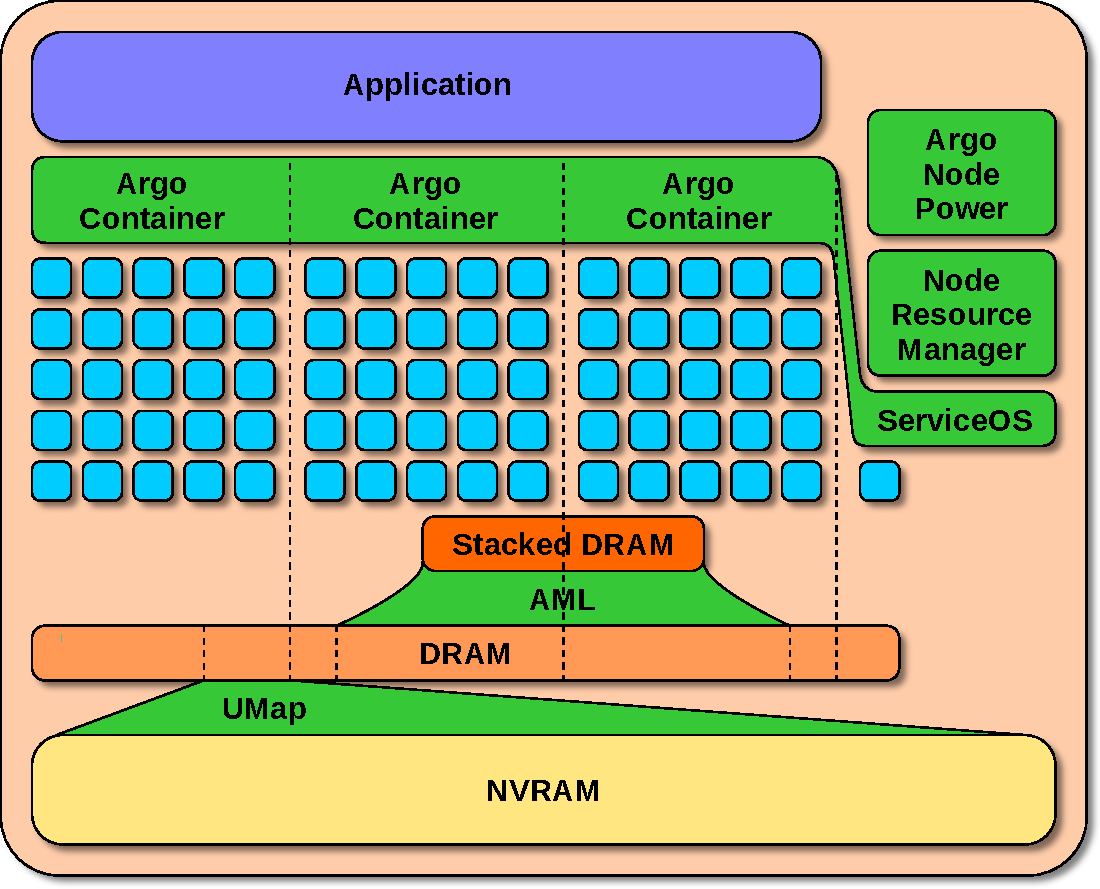
\includegraphics[height=.15\textheight]{projects/2.3.5-Ecosystem/2.3.5.05-Argo/argo-node}
\caption{Global and node-local components of the Argo software stack and
 interactions between them and the surrounding HPC system components.}
\end{figure}


\paragraph{Next Steps}

We plan to investigate different power management policies,
particularly demand response, which is becoming a crucial feature for
data centers, allowing to reduce the power consumption of servers
without killing running applications or shutting down nodes.
We plan to continue the 
development of power-aware versions of SLURM and Flux, and enable the path toward  
integration with GEOPM and NRM. 

We plan to improve the control loop inside the NRM to take into account I/O and
memory interference when placing containers on a node. We are also working on
making the NRM implementation compatible with Singularity.

We plan to improve the performance of UMap and demonstrate it with an
astronomy application having hundreds of files.
%
We plan to port applications to AML and integrate with runtime projects like
BOLT or PaRSEC for efficient use of Knights Landing memory using our
scratchpad.
